\chapter{Arquitetura de dados}\label{arquitetura-de-dados}

\section{UC como entidade de análise e NIO como ativo físico}\label{uc-como-entidade-de-anuxe1lise-e-nio-como-ativo-fuxedsico}

A telemetria é produzida por um medidor físico, identificado por NIO, mas o objeto comercial e operacional é a Unidade Consumidora. A hipótese simplificadora

\begin{quote}
\textbf{Hipótese simplificadora:} \texttt{1~UC~=~1~NIO~=~1~série}.
\end{quote}

não se mantém ao longo do tempo. Medidores são substituídos, podem mudar de cadência, podem reiniciar registradores e podem ser reutilizados.

A série da UC deve, portanto, ser reconstruída a partir do histórico de instalações:

\[X_u(t)=\sum_k \mathbf{1}[t\in I_{u,k}]Y_k(t),\]

onde \(Y_k(t)\) é a série do medidor \(k\) e \(I_{u,k}\) é seu intervalo de vigência na UC \(u\).

A expressão representa a composição de grandezas aditivas em intervalos de vigência não sobrepostos. Para grandezas instantâneas, como tensão e corrente, devem ser resolvidos os conflitos de atribuição antes de formar a série, sem somar indiscriminadamente leituras de equipamentos distintos. No dia de troca, a solução precisa admitir a coexistência de dois equipamentos durante partes distintas do dia. Registradores acumulados devem ser diferenciados por medidor antes da fusão em nível de UC.

\section{Camadas semânticas}\label{camadas-semuxe2nticas}

A arquitetura de dados é organizada em entidades com granularidades explícitas:

\begin{itemize}
\item
  \texttt{uc\_context}: atributos cadastrais e contextuais da UC;
\item
  \path{meter_installation_history}: vínculo UC-NIO com vigência;
\item
  \path{electrical_hierarchy}: subestação, alimentador, transformador/posto e localização;
\item
  \texttt{ami\_interval}: grandezas intervalares;
\item
  \texttt{ami\_instantaneous}: grandezas instantâneas;
\item
  \texttt{ami\_registers}: registradores acumulados;
\item
  \texttt{alarm\_events}: alarmes e eventos assíncronos.
\end{itemize}

O dataset de modelagem utiliza o grão conceitual

\[UC \times cutoff\_date.\]

Cada linha representa o estado conhecido de uma UC até uma data de corte. As colunas são separadas em:

\begin{itemize}
\item
  \texttt{id\_\_*}: identificadores, fora de \(X\);
\item
  \texttt{meta\_\_*}: tempo, qualidade, gating e controle;
\item
  \texttt{x\_\_*}: atributos permitidos aos modelos;
\item
  \texttt{y\_\_*}: alvos, quando existirem e forem validados.
\end{itemize}

Essa convenção reduz a chance de inclusão acidental de identificadores, metadados futuros ou targets dentro do vetor de treinamento.

\section{Temporalidade e vazamento temporal}\label{temporalidade-e-vazamento temporal}

A validação do pipeline exige distinguir tempo de medição, tempo de ocorrência do evento, tempo de recepção e tempo de disponibilidade para a análise. Em uma avaliação online, uma observação só pode ser utilizada se estivesse disponível no corte simulado.

As principais formas de vazamento temporal consideradas são:

\begin{itemize}
\item
  uso de dados posteriores ao corte;
\item
  uso de cadastro atual para representar estado histórico sem vigência;
\item
  ajuste de scaler, imputer ou encoder com dados do teste;
\item
  utilização de target ou proxy direto do target nos atributos;
\item
  construção de janelas que atravessam o período reservado para avaliação;
\item
  sobreposição excessiva entre janelas que cria dependência não tratada.
\end{itemize}

\section{Extração inteligente e processamento em escala}\label{extrauxe7uxe3o-inteligente-e-processamento-em-escala}

A plataforma não pressupõe que todos os dados estejam disponíveis em uma única tabela ou que uma extração de longo período possa ser mantida integralmente em memória. A ingestão foi desenhada para trabalhar em ciclos independentes por dia e por lote de medidores, permitindo que o estado do Data Lake determine o trabalho ainda necessário.

A chamada \textbf{sincronização inteligente} realiza três funções: identifica as partições temporais já consolidadas, detecta lacunas intermediárias e calcula o intervalo que ainda precisa ser extraído até o último dia completo. Com isso, uma execução interrompida não precisa ser reiniciada desde o início. Dias corretamente persistidos continuam sendo parte válida do histórico.

A extração pode ser acionada em quatro granularidades operacionais:

\begin{itemize}
\item
  dia de referência isolado;
\item
  período histórico definido pelo usuário;
\item
  alimentador específico;
\item
  \emph{auto-backfill} até o último dia completo.
\end{itemize}

No acesso ao Oracle, os identificadores são divididos em lotes e as conexões dos \emph{workers} são reutilizadas. Essa estratégia evita tanto consultas monolíticas que pressionam memória do banco quanto o custo de criar uma nova sessão a cada lote. O acompanhamento é apresentado em tempo real pela TUI por uma fila geral e barras individuais de \emph{workers}.

\section{Polars, execução lazy e persistência por sinking}\label{polars-execuuxe7uxe3o-lazy-e-persistuxeancia-por-sinking}

O volume de telemetria torna inadequado depender de concatenações sucessivas de DataFrames Python materializados integralmente em RAM. O pipeline utiliza Polars para privilegiar operações colunares e um plano de transformação \emph{lazy}. Sempre que a transformação permite, o resultado é materializado diretamente em disco por mecanismos de \emph{sinking}, como \texttt{sink\_parquet()} e \texttt{sink\_csv()}.

O propósito de \texttt{sink} não é apenas acelerar o processamento. Ele altera a tolerância a falhas do sistema. Em vez de exigir que um período completo termine para produzir um único artefato, cada partição diária consolidada torna-se imediatamente persistente e reutilizável. Assim, uma falha de rede, interrupção manual ou reinício da máquina não invalida os dias já concluídos.

Essa estratégia estabelece três propriedades importantes:

\begin{enumerate}
\def\labelenumi{\arabic{enumi}.}
\item
  \textbf{bounded memory:} o tamanho do histórico não precisa crescer proporcionalmente ao uso de RAM;
\item
  \textbf{checkpoint natural:} o próprio particionamento diário funciona como ponto de recuperação;
\item
  \textbf{resultados parciais auditáveis:} partes concluídas podem ser verificadas antes de toda a campanha terminar.
\end{enumerate}

A escolha por Parquet fornece compressão e leitura colunar eficiente, enquanto a exportação opcional em CSV preserva interoperabilidade com ferramentas externas. A TUI também permite sincronizar formatos ausentes sem repetir a consulta ao banco corporativo.

\section{Continuidade temporal e auditoria do Data Lake}\label{continuidade-temporal-e-auditoria-do-data-lake}

Uma série temporal só pode ser analisada corretamente quando se conhece também sua ausência. Por isso, a plataforma mantém um calendário mensal de continuidade. Cada dia é classificado conforme a existência das partições esperadas e, quando aplicável, conforme a presença dos formatos Parquet e CSV.

O calendário tem função metodológica: ele impede que uma lacuna de extração seja confundida com ausência de medição da UC. Também tem função operacional, pois permite ao usuário identificar rapidamente períodos incompletos e acionar \emph{backfill} ou sincronização de formatos.

Além do calendário, a aplicação executa auditorias de saúde do Data Lake. As verificações incluem presença de partições, contratos de schema, contagens, chaves esperadas, disponibilidade das camadas necessárias ao treinamento e execução da suíte de testes. O resultado é persistido em relatório de saúde com estados como \texttt{HEALTHY}, \texttt{WARNING}, \texttt{INCOMPLETE} e \texttt{CRITICAL}.

\section{Arquitetura geral da aplicação}\label{arquitetura-geral-da-aplicauxe7uxe3o}

A Figura \ref{fig:app_arch} resume o encadeamento entre ingestão, governança, modelagem e uso operacional. A TUI atua como camada de orquestração da engenharia; a interface web é tratada como camada de consumo analítico e acompanhamento das prioridades.

A arquitetura representada na figura separa fontes transacionais, artefatos persistidos, treinamento e apresentação. Essa organização é relevante porque uma anomalia exibida no Cockpit precisa ser reconstituída até o arquivo e o instante de origem; a figura não representa um fluxo único e atômico, pois cada estágio possui seus próprios checkpoints e verificações.

\begin{figure}[htbp]
\centering
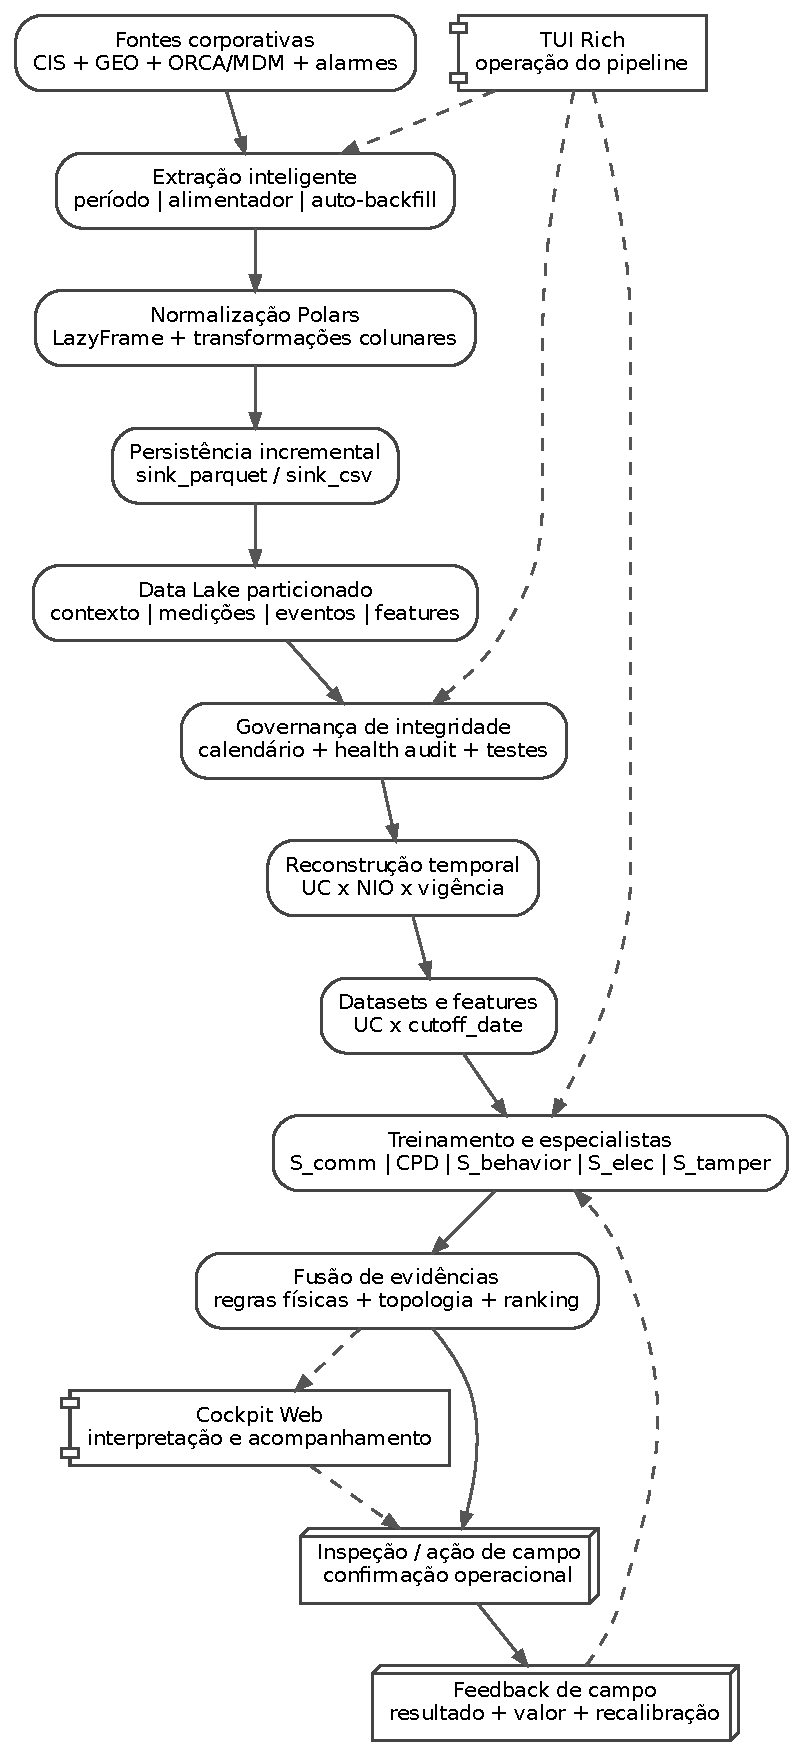
\includegraphics[width=0.94\textwidth,height=0.54\textheight,keepaspectratio]{figures/app_architecture.pdf}
\caption{Arquitetura geral da aplicação e perspectiva de realimentação por resultados de campo.}\label{fig:app_arch}
\par\small Fonte: elaboração própria.
\end{figure}
